% $Id$
% ---------------------------------------------------------------------------
%
% Copyright (c) 2008 Interlegis
%
% This is part of the relatorio-modelo.
%
% relatorio-modelo is free software; you can redistribute it and/or
% modify it under the terms of the GNU General Public License as
% published by the Free Software Foundation; either version 3 of the
% License, or (at your option) any later version.
%
% relatorio-modelo is distributed in the hope that it will be useful,
% but WITHOUT ANY WARRANTY; without even the implied warranty of
% MERCHANTABILITY or FITNESS FOR A PARTICULAR PURPOSE. See the GNU
% General Public License for more details.
%
% You should have received a copy of the GNU General Public License
% along with this program; see the file COPYING.  If not, see
% <http://www.gnu.org/licenses/>.
%

\documentclass[a4paper,12pt]{article}
\textheight 22.5cm
\usepackage[brazil]{babel}      % suporte ao portugues brasil
\usepackage[utf8]{inputenc}     % Codificacao dos caracteres (use a
                                % codificacao latin1 caso seu
                                % sistema/editor nao suporte utf8).
\usepackage[T1]{fontenc}
\usepackage{indentfirst}        % indenta o primeiro paragrafo 
\usepackage{graphicx}           % uso para imagens
\usepackage{dsfont}             % fonte

\usepackage{fancyhdr}           % permite alterar o cabecalho
\pagestyle{fancy}               % configura o estilo padrao

\newcommand{\titulo}{Produto: Webscan}
\newcommand{\subtitulo}{Relatório II}
\newcommand{\subsubtitulo}{Programas desenvolvidos, testados e documentados}
\newcommand{\autor}{Sérgio Oliveira Campos}
\newcommand{\numcontrato}{2008/000514} % Número do contrato caso seja consultor.
                % novos comandos

\usepackage[pdftex,%            % formatacao no PDF
pdfauthor={\autor},%
pdftitle={\titulo - \subtitulo},%
]{hyperref}
\hypersetup{backref=true,pdfpagemode=UseOutlines,colorlinks=true,
  breaklinks=true,hyperindex,linkcolor=blue,anchorcolor=black,
  citecolor=blue,filecolor=magenta,menucolor=red,pagecolor=red,
  urlcolor=cyan,bookmarks=true,bookmarksopen=true,pdfpagelayout=SinglePage,
  pdfpagetransition=Dissolve}


\begin{document}
% $Id$
% ---------------------------------------------------------------------------
%
%  This is part of the relatorio-modelo.
%  Copyright (C) 2008 Interlegis
%  See the file relatorio.tex for copying conditions.
%

\lhead {
  \begin{picture}(0,0) 
    
\includegraphics[scale=0.65]{imagens/cabecalho.pdf} 
  \end{picture} 
}
\chead{}
\rhead{}
\renewcommand{\headrulewidth}{0pt}

%
% Local variables:
%   mode: flyspell
%   TeX-master: "relatorio.tex"
% End:
%

\textsf{\vspace{7.5cm}}
\begin{center}
	\noindent
	\huge{
		\textbf{\titulo}
	} \\
	\Large{
		\textbf{\subtitulo}
	}

	\vspace{8cm}

	\large{
		\textbf{\autor}\\
		\textsf{Contrato N$^{\circ}$: \ncontrato}\\
	}
\end{center}
\cfoot{\large{\cidade, \data}}


% configura o rodape do conteudo pre-textual para numeros romanos
\clearpage
\cfoot{\thepage}
\setcounter{page}{1}
\pagenumbering{Roman}

\tableofcontents
\listoffigures
\listoftables

% configura o rodape das paginas de conteudo para numeros convencionais
\clearpage
\setcounter{page}{1}
\pagenumbering{arabic}

% conteudo
\section{Introdução}
\label{sec:intro}

Durante a primeira fase da elaboração do projeto {\it webscan}, foram realizadas as seguintes atividades:

\begin{description}
    \item[Casos de uso: ] Nessa atividade, descrita na seção \ref{sec:casos_de_uso}, foram elaborados diagramas de casos de uso, representando as principais interações entre atores e o sistema. Também foram elaborados os casos de uso completo-abstrato, de forma a dar detalhamento a cada caso de uso contido no diagrama;
    \item[Modelagem de dados: ] A modelagem de dados do projeto foi realizada para dar uma visão geral dos dados que serão tratados, e, como eles se relacionam entre si. A seção \ref{sec:modelo_de_dados} apresenta o resultado obtido desse trabalho realizado. 
    \item[Interface: ] Para essa atividade, descrita com mais detalhes na seção \ref{sec:mockups}, foram elaboradas as candidatas às telas de interface do sistema ({\it mockups} e também o curso de ações que um usuário pode realizar {\it storyboards};
    \item[Elaboração dos {\it Web Services}: ] Essa atividade consistiu na
        espeficação dos métodos que compõe a interface de comunicação da
        aplicação com outros sistemas. Toda a especificação está disponível
        na seção \ref{sec:web_services}. 
    \item[Pesquisa de bibliotecas: ] Essa atividade (apresentada nas seções \ref{sec:pesquisa_libs} e \ref{sec:pesquisa_ocr}) consistiu na realização de uma pesquisa sobre as bibliotecas de digitalização e de reconhecimento de textos respectivamente.

\end{description}

\subsection{Terminologia}

\subsubsection{Atividade de Desenvolvimento}
Atividade de desenvolvimento se refere à quantidade de escritas (ou seja, código sendo atualizado/adicionado) em um sistema de controle de versões, quando disponível.

\begin{description}
    \item[Alta:] diversas atividades no último mês.
    \item[Baixa:] algumas atividades ao longo dos últimos 3 meses.
    \item[Parado:] não houve nenhuma atividade de escrita nos últimos 6 meses.
\end{description}

\subsubsection{OCR - Optical Character Recognition}

O OCR (Optical Character Recognition), ou Reconhecimento Óptico de Caracteres, 
é a tecnologia responsável pela obtenção de texto apartir de uma imagem. Durante
este projeto a tecnologia será empregada para gerar documentos indexáveis\footnote{Documentos indexáveis: Que
podem ser encontrados pelo sistema de busca}.

\subsubsection{JSON}
Algumas vezes é necessário que uma pequena informação seja transmitida entre aplicações, e o formato XML acaba
burocratizando demasiadamente este processo. Outro cenário é o de múltiplas requisições em um curto espaço de
tempo, que leva o cliente e o servidor a uma sobrecarga para executar o \emph{parser}, além de um uso de
excessivo da banda para a transmissão dos dados.

A padronização de um formato Javascript para a transferencia de dados poderia ser uma alternativa para
solucionar estes problemas, e foi por isso que no ano de 2002 \emph{Douglas Crockford}, engenheiro da
\emph{Yahoo! Inc} propôs o formato JSON.

O principal objetivo era criar um padrão para troca de dados utilizando código javascript, ou seja, em forma
textual, gerando o mínimo de texto possível, o que tornaria o formato leve e ao mesmo tempo fácil de ser
interpretado pelo navegador. Para isso algumas assertivas foram seguidas:

\begin{itemize}
    \item Não poderia ser uma linguagem de marcação;
    \item Não seria um formato de documento;
    \item Não permitiria a representação de funções;
    \item Não permitiria a representação de estruturas cíclicas.
\end{itemize}

No ano de 2006 o formato foi oficializado pelo \emph{Network Working Group} e apresentado oficialmente a
comunidade durante a conferencia \textbf{XML 2006}.

O padrão apresentado é basicamente composto de um objeto (Figura \ref{fig:json_obj}) que possuí uma \emph{string}
descritiva e o seu valor, onde o seu valor pode assumir os formatos:

\begin{itemize}
    \item \emph{String}
    \item Número
    \item Vetor
    \item Objeto
    \item true, false e null
\end{itemize}

\begin{figure}[ht]
\begin{center}
\scalebox{0.6} {
    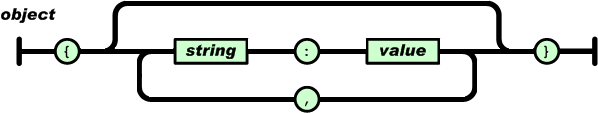
\includegraphics{img/json_obj.png}}
\end{center}
  \caption{Objeto JSON}
  \label{fig:json_obj}
\end{figure}

As definições detalhadas de cada um dos tipos e exemplos de código podem ser encontrados no site
http://www.json.org/.

\subsubsection{Web Services}

A W3C \footnote{http://www.w3c.org/} define \emph{web services} como um padrão que provê a
interoperabilidade entre duas aplicações de software, rodando sob diferentes plataformas e/ou
frameworks.
A interoperabilidade fornecida pelos \emph{web services} é disponibilizada por meio de funções
ou mesmo objetos na web, de forma que estes possam ser chamados através de um \emph{HTTP
request} e sua resposta retornada através de um \emph{HTTP response}.
Para que uma aplicação consiga se comunicar com a outra é necessário que ela conheça
e entenda o formato de entrada e saída de dados; para isso, costuma ser utilizado XML ou JSON.
Outro problema é que a aplicação deve saber qual o tipo de dados de um determinado
valor que chega a ela, e como ela implementa este valor. Este problema pode ser resolvido
de formas distintas; uma delas é a especificação trazer as informações necessárias; a outra
é o uso de um arquivo que trás esse tipo de informação, te tal forma que a aplicação
apenas leia este arquivo e faça as conversões necessárias. 


\section{Instalação}
\label{sec:instalacao}
Este capítulo descreve os passos para a instalação do módulo daemon do
{\it webscan}. O módulo UI não exige instalação e por esse motivo não

Estas instruções estão divididas em 2 seções que descrevem os
procedimentos de instalação nos sistemas Linux e Windows respectivamente.

Em ambos sistemas a instalação dos drivers específicos dos scanners que 
serão utilizados é necessária para que software trabalhe corretamente.

\subsection{Linux}
Esta seção cobre a instalação do produto {\it webscan} na distribuição
Ubuntu e outras que compartilham o mesmo tipo de gerenciamento de pacotes.

As linhas de comando apresentadas nesta seção poderão iniciar com `\#' ou
`\$'; quando iniciadas com `\#' significa que elas precisam ser executadas 
com super-usuário (ou root), caso contrário um usuário convencional será
suficiente.

\subsubsection{Pré-Requisitos}
Boa parte das dependências do {\it webscan} podem ser instaladas através 
do software apt-get executando-se o comando:

\begin{verbatim}
 # apt-get install [nome_do_pacote nome_de_outro_pacote]
\end{verbatim}

Os pacotes necessários são:

\begin{itemize}
    \item python
    \item python-imaging
    \item python-imaging-sane
    \item python-setuptools
    \item python-simplejson
\end{itemize}

Após instalados os pacotes do sistema operacional será necessária a 
instalação do Django. Baixe a versão 1.0 em:
\begin{verbatim}
http://www.djangoproject.com/
\end{verbatim}

Após baixar o pacote do Django a instalação deve ser realizada com as 
seguintes linhas de comando:
\begin{verbatim}
 $ tar xzvf Django-1.0.tar.gz
 $ cd Django-1.0
 # python setup.py install
\end{verbatim}

\subsubsection{Módulo daemon}
Para instalar o módulo daemon será necessário a cópia do 
código-fonte para o servidor onde o scanner será utilizado.

O código-fonte pode ser obtido no CD que segue junto a este
relatório. A versão atualizada deste código também pode ser encontrada
no repositório do projeto Interlegis em:
\begin{verbatim}
http://repositorio.interlegis.gov.br/digidoc/trunk/
\end{verbatim}
 

\subsection{Windows}

\section{Utilização}
\label{sec:utilizacao}

\section{Glossário}

\subsection{Atividade de Desenvolvimento:}
Atividade de desenvolvimento se refere à quantidade de escritas (ou seja, código sendo atualizado/adicionado) em um sistema de controle de versões, quando disponível.

\begin{description}
	\item[Alta:] diversas atividades no último mês.
	\item[Baixa:] algumas atividades ao longo dos últimos 3 meses.
	\item[Parado:] não houve nenhuma atividade de escrita nos últimos 6 meses.
\end{description}

\end{document}
